\documentclass[10pt]{beamer}
\usepackage[utf8]{inputenc}
\usepackage{xeCJK}
\usepackage{graphicx}
\usepackage{mathtools}
\usepackage{utopia} 
\usepackage{geometry}
\usepackage{booktabs}
\usepackage{multirow}
\usepackage{array}

\usetheme{CambridgeUS}
\usecolortheme{dolphin}

% HKUST Colors
\definecolor{hkustyellow}{RGB}{167, 131, 55}
\definecolor{hkustblue}{RGB}{0, 56, 116}
\definecolor{hkustred}{RGB}{209, 51, 59}
\setbeamercolor*{palette primary}{bg=hkustblue, fg = white}
\setbeamercolor*{palette secondary}{bg=hkustred, fg = white}
\setbeamercolor*{palette tertiary}{bg=hkustyellow, fg = white}
\setbeamercolor*{titlelike}{fg=hkustblue}
\setbeamercolor*{title}{bg=hkustblue, fg = white}
\setbeamercolor*{item}{fg=hkustblue}
\setbeamercolor*{caption name}{fg=hkustblue}
\usefonttheme{professionalfonts}

% --- Background and Title Info ---
\titlegraphic{
\includegraphics[height=1.5cm]{UST.png}}
\setbeamerfont{title}{size=\large}
\setbeamerfont{subtitle}{size=\small}
\setbeamerfont{author}{size=\small}
\setbeamerfont{date}{size=\small}
\setbeamerfont{institute}{size=\small}
\setbeamertemplate{background}{%
    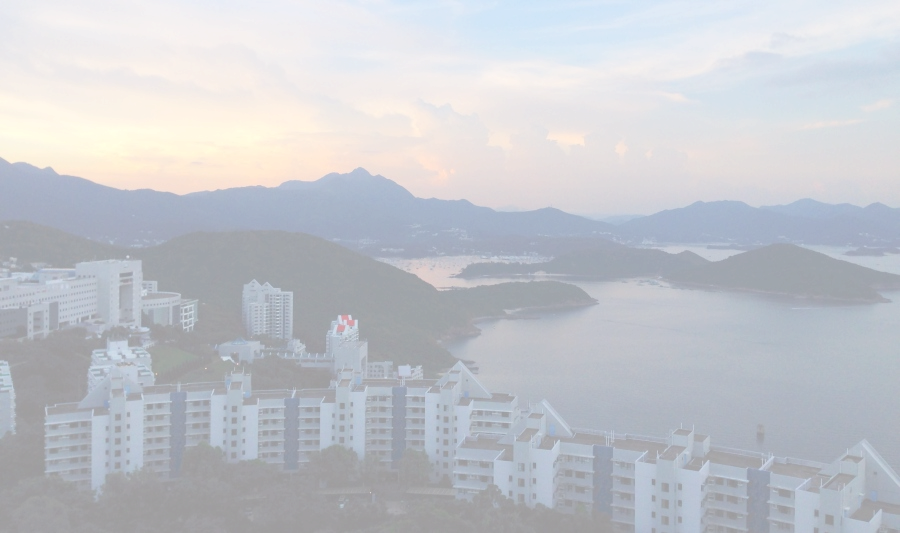
\includegraphics[width=\paperwidth,height=\paperheight]{ustscene.png}
}

\title[ML for NPA Repayment Prediction]{\textrm{\textbf{Machine Learning for Non-Performing Asset Repayment Probability Prediction and Strategy Optimization}}}
\subtitle{\textrm{A Comparative Study: Traditional ML vs. LLM on Imbalanced Portfolios}}
\author[ZHU TIANYI]{\textrm{Student: ZHU TIANYI (21229582)\\[0.5ex] Supervisor: Mr. Hanson WONG}}
\institute[HKUST]{\textrm{The Hong Kong University of Science and Technology}}
\date[May 2026]{\textrm{Academic Defense -- May 2026}}

\AtBeginSection[]{
  \begin{frame}
  \vfill
  \centering
  \begin{beamercolorbox}[sep=8pt,center,shadow=true,rounded=true]{title}
    \usebeamerfont{title}\insertsectionhead\par%
  \end{beamercolorbox}
  \vfill
  \end{frame}
}

\begin{document}

% 1. Title Page
\frame{\titlepage}

% 2. Table of Contents
\begin{frame}{\textrm{Presentation Outline}}
\tableofcontents[hideallsubsections]
\end{frame}

% ==========================================
\section{I. Introduction}
% ==========================================

% 3. Background
\begin{frame}{\textrm{Background and Problem Statement}}
    \begin{itemize}
        \item \textbf{Non-Performing Assets (NPAs):} Significant risk for global financial institutions.
        \item \textbf{Operational Challenge:} How to allocate limited collection resources across millions of delinquent accounts?
        \item \textbf{Core Statistical Problem:} \textbf{Prediction under extreme class imbalance}.
        \item \textbf{The Signal:} Only 5--15\% of accounts repay; identifying this minority is critical for profitability.
        \item \textbf{Transition:} Shifting from heuristic "Uniform Treatment" to data-driven "Precision Targeting."
    \end{itemize}
\end{frame}

% 4. Objectives
\begin{frame}{\textrm{Research Objectives (O1 -- O4)}}
    \begin{enumerate}
        \item \textbf{Develop \& Compare:} Implement four ML models (LR, RF, XGBoost, MLP v2) for binary repayment prediction.
        \item \textbf{Multi-dimensional Evaluation:} Assess ranking power (AUC), calibration (Brier Score), and economic ROI.
        \item \textbf{Queue Optimization:} Design a tiered collection strategy (Agent/Dialer/SMS) based on calibrated probabilities.
        \item \textbf{AI Benchmarking:} Test if "asking an AI" (LLMs) can match specialized ML models for tabular financial tasks.
    \end{enumerate}
\end{frame}

% ==========================================
\section{II. Student's Unique Contributions}
% ==========================================

% 5. Contributions - Pipeline
\begin{frame}{\textrm{Contribution 1: End-to-End Pipeline Design}}
    \begin{itemize}
        \item \textbf{Domain-Aware Missing Value Strategy:} Interpreted null values in \texttt{last\_pay\_date} as "Never Paid" (Predictive Missingness) rather than simple imputation.
        \item \textbf{Tailored Architectures:} Custom preprocessing for each model family (e.g., $z$-score for MLP, ordinal encoding for Tree-based).
        \item \textbf{Robust Calibration:} Integration of 5-fold out-of-fold Platt Scaling to ensure probability reliability.
    \end{itemize}
\end{frame}

% 6. Contributions - LLM & Strategy
\begin{frame}{\textrm{Contribution 2: Strategy \& Benchmarking}}
    \begin{itemize}
        \item \textbf{LLM-vs-ML Benchmark:} Systematic evaluation of Zero-shot, Few-shot, and Fine-tuned LLMs against traditional classifiers.
        \item \textbf{Economic Strategy Module:} Formulation of a 4-tier allocation framework with explicit cost/capacity constraints.
        \item \textbf{Inverse Relationship Discovery:} Identifying that resources are most efficient on low-balance accounts ($<$HKD 25k).
    \end{itemize}
\end{frame}

% ==========================================
\section{III. Data and Methodology}
% ==========================================

% 7. Data Schema
\begin{frame}{\textrm{Dataset Schema (16,048 Accounts)}}
\centering
\scriptsize
\begin{tabular}{@{}llp{5.5cm}@{}}
\toprule
\textbf{Feature} & \textbf{Type} & \textbf{Description}\\
\midrule
\texttt{loan\_type} & Cat. & Product category (Credit Card, Loan, etc.)\\
\texttt{purchased\_bal\_gp} & Ord. & Balance bucket group (8 levels)\\
\texttt{birth\_yr} & Int & Borrower birth year (1946--1987)\\
\texttt{last\_act\_closing\_m} & Float & Months since last activity\\
\texttt{open\_closing\_m} & Float & Account vintage in months\\
\texttt{last\_pay\_date\_m} & Float & Months since last payment (imputed sentinel)\\
\texttt{balance\_proxy} & Float & Outstanding balance amount (HKD)\\
\texttt{multiple\_acct} & Cat. & Holds multiple accounts? (Y/N)\\
\midrule
\texttt{payer\_3yr} & \textbf{Target} & \textbf{Repaid within 3 years? (Positive Rate: 9.65\%)}\\
\bottomrule
\end{tabular}
\end{frame}

% 8. Preprocessing
\begin{frame}{\textrm{Preprocessing Pipeline}}
    \begin{itemize}
        \item \textbf{Sentinel Flagging:} Created \texttt{never\_paid\_flag} to capture semantic meaning of missing dates.
        \item \textbf{Encoding:} One-hot encoding for LR/MLP; Ordinal encoding for RF/XGBoost.
        \item \textbf{Splitting:} Training ($M$, 75\%, $N=12{,}036$) and Test ($T$, 25\%, $N=4{,}012$).
        \item \textbf{Calibration Holdout:} 20\% of $M$ reserved strictly for Platt Scaling parameter fitting.
    \end{itemize}
\end{frame}

% 9. Architectures - Traditional
\begin{frame}{\textrm{Traditional Models: LR, RF, XGBoost}}
    \begin{itemize}
        \item \textbf{Logistic Regression (LR):} Linear baseline, $\ell_2$ penalty, balanced class weights.
        \item \textbf{Random Forest (RF):} 500 trees, capturing non-linear interactions, max depth 12.
        \item \textbf{XGBoost (Champion Ranker):} 
        \[ \mathcal{L} = \sum \ell(y_i, \hat{y}_i) + \sum \Omega(f_k) \]
        Gradient boosting with \texttt{scale\_pos\_weight} $\approx$ 9.2.
    \end{itemize}
\end{frame}

% 10. Architecture - MLP v2
\begin{frame}{\textrm{Advanced Architecture: Multi-Layer Perceptron v2}}
    \textbf{Design Features:}
    \begin{itemize}
        \item \textbf{Residual Block:} $\mathbf{h}_{\ell+1} = \text{Swish}(\mathbf{W}_2 \sigma(\mathbf{W}_1 \mathbf{h}_\ell) + \mathbf{b}_2 + \mathbf{h}_\ell)$.
        \item \textbf{Feature Interaction Layer:} Explicit pairwise product modeling for tabular patterns.
        \item \textbf{Training:} AdamW optimizer, label smoothing ($\alpha=0.03$), gradient clipping.
    \end{itemize}
\end{frame}

% 11. Calibration - Platt
\begin{frame}{\textrm{Probability Calibration: Platt Scaling}}
    \textbf{The Problem:} XGBoost margin scores are not true probabilities.
    \begin{block}{The Formula}
        \[ P_{\text{calibrated}}(y=1|s) = \frac{1}{1 + \exp(A \cdot s + B)} \]
    \end{block}
    \begin{itemize}
        \item Parameters $(A, B)$ fit via maximum likelihood.
        \item Vital for economic allocation where threshold depends on absolute probability.
    \end{itemize}
\end{frame}

% ==========================================
\section{IV. Results and Analysis}
% ==========================================

% 12. Main Performance Table
\begin{frame}{\textrm{Model Performance Comparison (Test Set)}}
\centering
\small
\begin{tabular}{lccccr}
\toprule
\textbf{Model} & \textbf{AUC} & \textbf{Brier} & \textbf{Recall} & \textbf{Net Recov.} & \textbf{ROI}\\
\midrule
\textbf{XGBoost} & \textbf{0.7305} & 0.0910 & 62.7\% & 1.270M & 25.4x\\
Random Forest & 0.7161 & 0.0855 & \textbf{75.4\%} & 1.241M & 24.8x\\
\textbf{Logistic Reg.} & 0.6994 & \textbf{0.0842} & 74.1\% & \textbf{1.468M} & \textbf{29.4x}\\
MLP v2 & 0.7063 & 0.0869 & 74.6\% & 1.405M & 28.1x\\
\bottomrule
\end{tabular}
\vfill
\begin{itemize}
    \item \textbf{Observation:} XGBoost leads in ranking, but \textbf{LR leads in economic Net Recovery} due to better calibration.
\end{itemize}
\end{frame}

% 13. Image: Model Comparison Graphs
\begin{frame}{\textrm{Discrimination vs. Calibration}}
\centering

\includegraphics[width=0.85\textwidth]{report_figures/fig1_model_comparison.png}
\vfill
\begin{itemize}
    \item \textbf{Left:} ROC-AUC (XGBoost superiority).
    \item \textbf{Right:} Brier Score (LR superiority in calibration).
\end{itemize}
\end{frame}

% 14. Image: ROC Curves
\begin{frame}{\textrm{ROC Curve Analysis}}
\centering

\includegraphics[width=0.7\textwidth]{report_figures/fig4_roc_curves.png}
\end{frame}

% 15. Image: Confusion Matrix
\begin{frame}{\textrm{Operational Accuracy (Confusion Matrices)}}
\centering

\includegraphics[width=0.65\textwidth]{report_figures/fig2_confusion_matrices.png}
\vfill
\begin{itemize}
    \item XGBoost produces the fewest False Positives (659), reducing wasted agent effort.
\end{itemize}
\end{frame}

% 16. Image: Feature Importance
\begin{frame}{\textrm{Permutation Feature Importance (XGBoost)}}
\centering

\includegraphics[width=0.8\textwidth]{report_figures/fig3_feature_importance.png}
\vfill
\begin{itemize}
    \item \textbf{Birth Year} is the dominant predictor, suggesting older borrowers exhibit different stability.
    \item \textbf{District} and \textbf{Balance} follow in importance.
\end{itemize}
\end{frame}

% 17. Image: Inverse Balance Relationship
\begin{frame}{\textrm{Inverse Balance-Repayment Relationship}}
\centering

\includegraphics[width=0.75\textwidth]{report_figures/fig6_balance_payer_rate.png}
\vfill
\begin{itemize}
    \item \textbf{Finding:} Lower balance accounts ($<$5k) have $\approx$ 25\% repayment rates.
    \item \textbf{Strategy Shift:} Focus SMS/Dialer resources on high-volume, low-balance accounts.
\end{itemize}
\end{frame}

% ==========================================
\section{V. Collection Strategy Optimization}
% ==========================================

% 18. Queue Allocation Table
\begin{frame}{\textrm{Optimized Queue Allocation Summary}}
\centering
\scriptsize
\begin{tabular}{lrrrr}
\toprule
\textbf{Tier} & \textbf{Accounts} & \textbf{Cost (HKD)} & \textbf{Net Recov.} & \textbf{ROI}\\
\midrule
Agent Call (High) & 722 & 61,370 & 1,085,006 & 17.7x\\
Auto-Dialer (Med) & 1,685 & 20,220 & 993,086 & 49.1x\\
SMS/Email (Low) & 1,203 & 1,805 & 190,469 & 105.6x\\
Write-off & 402 & 0 & 0 & --\\
\midrule
\textbf{Total} & \textbf{4,012} & \textbf{83,395} & \textbf{2,268,561} & \textbf{27.2x}\\
\bottomrule
\end{tabular}
\vfill
\begin{itemize}
    \item Projected \textbf{HKD 2.27 Million} recovery on a small HKD 83k budget.
\end{itemize}
\end{frame}

% 19. Image: Queue Allocation Visualization
\begin{frame}{\textrm{Strategy Concentration}}
\centering

\includegraphics[width=0.85\textwidth]{report_figures/fig5_queue_allocation.png}
\vfill
\begin{itemize}
    \item \textbf{Pareto Effect:} Top 20\% of accounts capture 50.6\% of total expected net recovery.
\end{itemize}
\end{frame}

% ==========================================
\section{VI. LLM Benchmark (Traditional vs. AI)}
% ==========================================

% 20. LLM Methodology
\begin{frame}{\textrm{Benchmarking "AI-as-Judge"}}
    \textbf{Seven Methods Evaluated:}
    \begin{itemize}
        \item \textbf{Heuristics:} Random Guess, Majority Class, Rule-Based.
        \item \textbf{Zero-Shot (GPT-4o):} No training, just natural language prompts.
        \item \textbf{Few-Shot (GPT-4o):} 5 exemplar accounts provided in prompt.
        \item \textbf{Fine-Tuned (FT):} GPT-4o-mini/LLaMA-3 trained on full dataset.
    \end{itemize}
    
    \vspace{0.2cm}
    \textbf{Prompt Design (Comprehensive Zero-Shot Example):}
    \vspace{-0.1cm}
    \begin{quote}
    \tiny % 使用极小号字体确保一页能装下
    \texttt{\textbf{Role:} You are an Expert Credit Risk Modeler and NPA Collection Strategist. You specialize in analyzing behavioral and demographic signals in highly imbalanced unsecured debt portfolios...}\\
    \texttt{\textbf{Task:} Evaluate the provided borrower profile and predict the precise probability ($P \in [0.000, 1.000]$) of them making a repayment within a 3-year window.}\\
    \texttt{\textbf{Domain Context:} 1) \textit{Age Dynamics}: older cohorts exhibit distinct default inertia. 2) \textit{Balance Paradox}: Micro-balances ($<$5K HKD) repay at $>25\%$, mega-balances ($>$200K HKD) approach $0\%$. 3) \textit{Missingness}: '999' in months since last payment indicates severe default risk.}\\
    \texttt{\textbf{Account Details:} Loan Type: \{loan\_type\} | Balance (HKD): \{balance\_proxy\} | Age: \{age\} | ... [Full Feature Space]}\\
    \texttt{\textbf{Instructions:} \textbf{[ANALYSIS]:} Write a concise 3-4 sentence Chain-of-Thought evaluating the combined risk factors. \textbf{[PREDICTION]:} Provide ONLY the numerical probability.}
    \end{quote}
\end{frame}

% 21. LLM Performance Table
\begin{frame}{\textrm{Benchmark Results: LLM vs. Traditional ML}}
\centering
\scriptsize
\begin{tabular}{lcccc}
\toprule
\textbf{Method} & \textbf{AUC} & \textbf{Brier} & \textbf{Net Recov.} & \textbf{ROI}\\
\midrule
Rule-Based Heuristic & 0.5620 & 0.0953 & 0.312M & 5.2x\\
GPT-4o Zero-Shot & 0.5940 & 0.1021 & 0.398M & 6.1x\\
FT GPT-4o-mini & \textbf{0.7120} & 0.0875 & 1.105M & 20.9x\\
\midrule
\textbf{Logistic Regression} & 0.6994 & \textbf{0.0842} & \textbf{1.468M} & \textbf{29.4x}\\
\textbf{XGBoost} & \textbf{0.7305} & 0.0910 & 1.270M & 25.4x\\
\bottomrule
\end{tabular}
\vfill
\begin{itemize}
    \item \textbf{Verdict:} Zero-shot LLMs are non-competitive. Even fine-tuned LLMs lag behind simple LR in profitability.
\end{itemize}
\end{frame}

% 22. Operational Comparison
\begin{frame}{\textrm{Operational Analysis: The "AI Tax"}}
\centering

\includegraphics[width=0.85\textwidth]{report_figures/fig12_llm_cost_benefit.png}
\vfill
\begin{itemize}
    \item \textbf{Latency:} ML (0.05ms) vs. LLM (2,500ms).
    \item \textbf{Cost:} API costs for LLM make it 1000x more expensive than local ML inference.
\end{itemize}
\end{frame}

% ==========================================
\section{VII. Conclusion}
% ==========================================

% 23. Summary of Findings
\begin{frame}{\textrm{Summary of Principal Findings}}
    \begin{itemize}
        \item \textbf{Ranking vs. Profit:} XGBoost is the best ranker, but Logistic Regression is the best profit-maker due to superior calibration.
        \item \textbf{Calibration is Mandatory:} Uncalibrated models lead to misallocated agent time.
        \item \textbf{Drivers:} Age and Balance are primary drivers; resources should shift to low-balance tiers.
        \item \textbf{LLM Maturity:} LLMs are not yet ready for high-throughput tabular prediction; specialized ML remains the gold standard.
    \end{itemize}
\end{frame}

% 24. Future Work
\begin{frame}{\textrm{Limitations and Future Work}}
    \begin{itemize}
        \item \textbf{Temporal Validation:} Future work needs time-series cross-validation.
        \item \textbf{Survival Analysis:} Predicting \textit{when} a debtor will pay, not just \textit{if}.
        \item \textbf{Hybrid Approach:} Using ML for prediction and LLMs for generating personalized customer explanations.
    \end{itemize}
\end{frame}

% 25. Thank You
\section*{}  
\begin{frame}
\textcolor{hkustblue}{\Huge{\center{\centerline{\textrm{\textbf{THANK YOU!}}}}}}
\vfill
\centering
\textbf{Questions and Discussion}
\end{frame}

\end{document}